\documentclass[11pt]{article}
\usepackage{mathptmx}
\usepackage{latexsym}
\usepackage{amsmath}
\usepackage{amssymb}
\usepackage{amsthm}
\usepackage{epsfig}
\usepackage{psfig}
\usepackage{graphicx}

\newcommand{\handout}[5]{
  \noindent
  \begin{center}
  \framebox{
    \vbox{
      \hbox to 5.78in { {\bf 6.851: Advanced Data Structures } \hfill #2 }
      \vspace{4mm}
      \hbox to 5.78in { {\Large \hfill #5  \hfill} }
      \vspace{2mm}
      \hbox to 5.78in { {\em #3 \hfill #4} }
    }
  }
  \end{center}
  \vspace*{4mm}
}

\newcommand{\lecture}[4]{\handout{#1}{#2}{#3}{Scribes: #4}{Lecture #1}}

\newtheorem{theorem}{Theorem}
\newtheorem{corollary}[theorem]{Corollary}
\newtheorem{lemma}[theorem]{Lemma}
\newtheorem{observation}[theorem]{Observation}
\newtheorem{proposition}[theorem]{Proposition}
\newtheorem{definition}[theorem]{Definition}
\newtheorem{claim}[theorem]{Claim}
\newtheorem{fact}[theorem]{Fact}
\newtheorem{assumption}[theorem]{Assumption}

% 1-inch margins, from fullpage.sty by H.Partl, Version 2, Dec. 15, 1988.
\topmargin 0pt
\advance \topmargin by -\headheight
\advance \topmargin by -\headsep
\textheight 8.9in
\oddsidemargin 0pt
\evensidemargin \oddsidemargin
\marginparwidth 0.5in
\textwidth 6.5in

\parindent 0in
\parskip 1.5ex
%\renewcommand{\baselinestretch}{1.25}

\begin{document}

\lecture{2 --- Februrary 9, 2012}{Spring 2012}{Prof.\ Erik Demaine}{Erek Speed and Wiktor Jakubiuk}

\section{Overview}

In previous lectures, we've discussed data structures that efficiently provided many nice properties. However, we have never discussed any data structures that provide the somewhat magical property of \emph{time travel}.

In this lecture we discuss temporal data structures, which will allow us to view and/or modify our data structure at various points in the past, in addition to its present state. The specific behaviors of these data structures are defined below.

\section{Temporal Data Structures}

There are two primary models of temporal data structures. The first, called persistence, is based on the branching-universe model of time travel. In this model, going back in time and making changes creates a new branch of the data structure that differs from the original branch. The second, called retroactivity, works on the idea of round-trip time travel. Here, a time traveller goes back in time, makes a change, and then returns to observe the effects of his or her change. This model gives us a there is a linear timeline with no branching.

\subsection{Persistence}

We begin by describing the levels of desired persistence. With data structure persistence, we would like to keep all versions of the data structure available for updates and queries. Each persistence level, however will vary based on where updates are allowed and how branches and nodes are modified and created.

\begin{enumerate}
\item{Partial Persistence} --
In this persistence model, we may query any previous version of the data structure, but we may only update the latest version. This implies a linear ordering among the versions.

\item{Full Persistence} --
In this model, both updates and queries are allowed on any version of the data structure. The versions here form of a branching tree.

\item{Confluent Persistence} --
In this model, we use combinators to combine input of $> 1$ previous versions to output a new single version. Rather than a branching tree, combinations of versions induce a DAG structure on the version graph.

\item{Functional Persistence} --
This model takes its name from functional programming where objects are immutable. The versions in this model are likewise immutable, so revisions do not alter the existing nodes in the data structure, but create new ones instead. Okasaki discusses these as well as other functional data structures in his book \cite{okasaki}.
\end{enumerate}

Each of the succeeding levels of persistence imply the preceding ones. That is, Functional Persistence $\implies$ Confluent Persistence $\implies$ Full Persistence $\implies$ Partial Persistence. Functional implies confluent because we simply use the combinators to append a new combined version. Confluent implies full if we do not use combinators. Lastly, full implies partial if we only update the most recent version.

\begin{figure}[h]
  \begin{center}
    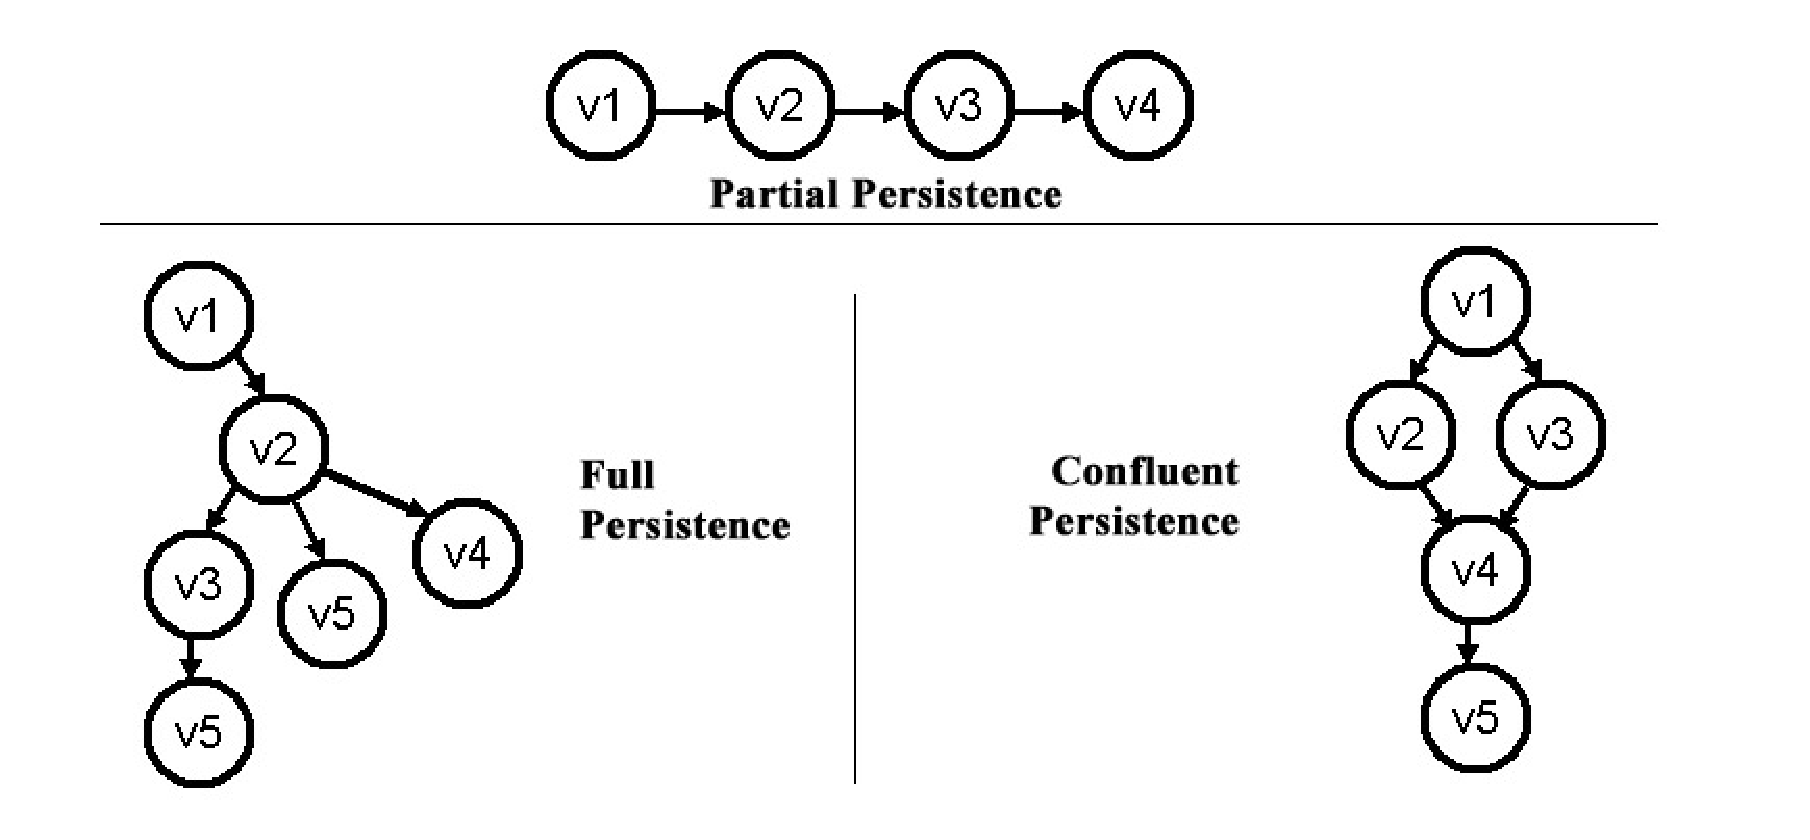
\includegraphics[width=6in]{types.pdf}
  \end{center}

  \caption{\small Abstract cartoons of the major persitence types.}
  \label{fig-label}
\end{figure}

\subsubsection{Partial Persistence}
This result is due to Driscoll, Sarnak, Sleator, and Tarjan \cite{dsst}.
We work within the pointer machine model and require $O(1)$ in-degree per node, meaning that $\leq p = O(1)$ nodes point to any node. Each node stores some data and a constant number of pointers to children, reverse pointers to parents, and version modification data (in a ``modification box''). To maintain partial persistence, each node stores a reverse pointer to the parent node representing the most recent version of the data structure. A modification can be thought of as the tuple $(time, field, value)$, consisting of the time of the modification, the field being modified, and the new value.\\
\\
An update on a field at some time $t$ can come across two cases:
\begin{itemize}
\item{The node has space} -- We can simply add the modification $(t, field, value)$ to the modification box. All subsequent accesses of this modified node will check the modification box to override any initial data stored in the node.
\item{The node is full} -- We make a copy of the node, but using only the latest values. That is, we overwrite one of the node�s fields with the value that was stored in the modification box, and make the modification box of the new node empty. We propagate this change up to node's ancestors as follows: each ancestor makes a modification to change its child pointer to the newly created node. If that ancestor's modification box happens to be full, then we copy that node and propagate up. These changes propagate until we stop at the root.
\end{itemize}

Using $\Phi = $ the number of full latest nodes, we can prove constant time amortized updates. Further study by Brodal \cite{brodal} has shown it to also be $O(1)$ in the worst case.

\subsubsection{Full Persistence}
This result is also due to \cite{dsst}. We again assume a pointer machine with $\leq p$ incoming pointers per node. We can speak of the version list, which is equivalent to a pre-order traversal of the version tree. Deitz and Sleator showed we can insert and compare the order of nodes in this so called list-order data structure (the version list) in $O(1)$ time \cite{dietz}. We will discuss this data structure in more depth in lecture 19. A related open question is whether we can support $O(1)$ worst-case full persistence?\\
\\
Each node can store up to $2p$ modifications. When a node is full, we split it into two roughly half-full nodes (like B-trees). Using $\Phi = $ the number of full nodes in all versions, we get $O(1)$ amortized cost. Each data structure node is represented by a linked list of nodes, and there's a second phase of the operation to update reverse pointers. Deitz developed a fully persistent array that can be achieved in $O(\lg \lg n)\ \times$ overhead in the word RAM model \cite{dietz1}.\\
{\bf OPEN:} Is there a matching lower bound for both full and partial persistence? This question may have been solved by P$\breve{a}$trascu et al. (unpublished).\\

\begin{figure}[h]
  \begin{center}
    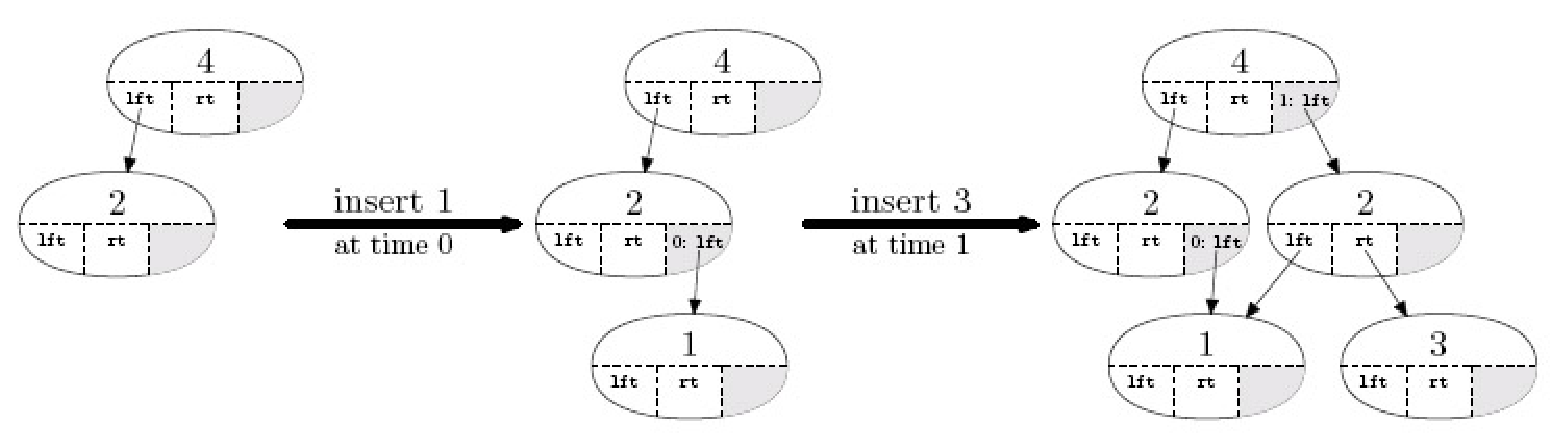
\includegraphics[width=6in]{ptree.pdf}
  \end{center}

  \caption{\small Persistence of a binary tree. We need a modification box the size of the in-degree of each data structure node (just one for trees).}
  \label{fig-label}
\end{figure}

\subsubsection{Confluent Persistence}

Confluent persistence has been explored in functional data structures \cite{okasaki}. Deques (double ended queues allowing stack and queue operations) with concatenation can be done in constant time per operation (Kaplan, Okasaki, and Tarjan \cite{kot}). We can create implicity exponential deques in polynomial time by recursively concatenating a node with itself. The general transformation due to Fiat and Kaplan \cite{fiat} is as follows:
\begin{itemize}
\item $d(v)$ = depth of node $v$ in version DAG
\item $e(v) = 1 + lg($ number of paths root to $v$)
\item overhead: $\lg($ number of updates $) + max_v(e(v))$
\item poor when $e(v) = 2^{u}$ where $u$ is the number of updates (see Figure 1). This is still exponentially better than the non-persistent model.
% add this figure from notes
\end{itemize}

{\bf OPEN:} When can you do better? Lists with split and concatenate? Trees? General pointer machine? Array with cut and paste? Special DAGs? Others?

\subsection{Retroactivity}
Retroactive data structures store a data structure under a sequence of operations. We would like to be able to go back in time, change an operation, and then observe the effects of that change in the current state of the data structure. The induced timeline is linear. Much of this work is due to Demaine, Iacono, and Langerman \cite{dil}.\\
\\
The allowed operations are
\begin{itemize}
\item{Insert($t, x$)} -- Retroactively do operation $x$ at time $t$
\item{Delete($t$)} -- Retroactively undo operation at time $t$	
\item{Query($t, x$)} -- Do query $x$ at time $t$
\end{itemize}

We define partial retroactivity as allowing queries at the present time and full retroactivity as allowing queries at any time.	Some cases of partial retroactivity are easy to implement. If updates are commutative: $x \circ y = y \circ x$, then we can support retroactive insertion of operations at no additional asymptotic cost (implement $Insert(t,x)$ by executing $x$ at the present time). If updates, in addition to being commutative, are also invertible: $x \circ x^{-1} = NOP$, then we can support partial retroactivity at no additional asymptotic cost ($Insert(t,x)$ by executing $x$ at the present time and $Delete(t)$ by executing $x^{-1}$ at the present time where $x^{-1}$ is the inverse of the operation at time $t$).

\subsubsection{The Rollback Method}
There are a few general transformations that we can prove bounds for. One is the rollback method, in which we perform a retroactive operation at $r$ time units in the past. We can do this with a factor of $r$ overhead by keeping a log of all updates done to the DS such that every change can be reversed. The rollback method needs an $\Omega(r)$ lower bound. To see this, we examine a data structure that maintains two values, $X$ and $Y$, both initialized to 0. We can perform the following operations on our data structure:
\begin{itemize}
	\item{set$X(x)$} -- Sets $X \leftarrow x$
	\item{add$Y(\Delta)$} -- Sets $Y \leftarrow Y + \Delta$
	\item{mult$XY$()} -- Sets $Y \leftarrow X \cdot Y$
  \item{query()} -- Returns $Y$
\end{itemize}
Consider the following sequence of operations: add$Y(a_n)$, mult$XY$(), add$Y(a_{n-1})$, mult$XY$(), ...,  add$Y(a_0)$. This is Horner's rule for evaluating the polynomial $p(x) = \sum_{i=0}^n a_i x^i$. Now suppose we perform $Insert(t=0,$ set$X(x_0))$ to change the $x$ value of the evaluated polynomial $x_0$. Frandsena, Hansen, and Miltersen in 2001 showed that evaluating a polynomial of degree $n$ requires $\Omega(n)$ time over any field, independent of any preprocessing of the $a_i$s. This holds in the ``history-independent algebraic decision tree'' model, which implies the same result for the integer RAM and generalized real RAM models \cite{fhm}. This is somewhat disappointing result because it says that in the retroactive model, we can't do any persistence maintenance that's better than just going back in time, performing the new operation, and then re-executing all of the operations in our history past that point.\\
\\
In the cell-probe model, Frandsena et al. also proved a lower bound of $\Omega(\sqrt{r/\lg r})$. They had a data structure that maintained $n$ words and supported arithmetic updates ($+/\cdot$). Computing a fast fourier transform takes $O(n \lg n)$ time, but changing one weights $w_i$ of the FFT needs $\Omega(\sqrt{n})$ time, from which we derive the $\Omega(\sqrt{r/\lg r})$ lower bound. An open question is whether the tightest cell-probe lower bound is $\Omega(\sqrt{r/\text{poly} \lg r})$.

\subsubsection{Priority Queues}
Let us turn our attention to partially retroactive priority queues. The defining features of priority queues is the delete-min() operation, which makes the set of operations on priority queues non-commutative. We can plot the status of our data structure in the plane. The $x$-axis represents time and $y$-axis represents key value. Every $insert(t,k)$ operation creates a horizontal ray that starts at point $(t,k)$ and shoots to the right. Every $delete$-$min()$ operation creates a vertical ray that starts at $(t,-\infty)$ and shoots upwards, stopping at the horizontal ray of the element it deletes. It turns the horizontal ray into a line segment with endspoints $(t,k)$ and $(d_k,k)$, where $d_k$ is the time of key $k$'s deletion. This creates nonintersecting upsidedown ``L'' shapes, where each L corresponds to an $insert$ and the $delete$-$min()$ that deletes it. Refer to Figure \ref{fig:bridges} for an animation.

\begin{figure*}[h]
  \centering
  \leavevmode
  \scalebox{.5}{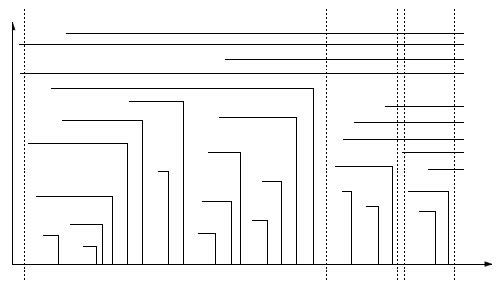
\includegraphics{bridges.png}}
  \caption{The ``L'' representation of a sequence of operations. Dotted horizontal lines represent \emph{bridges}. \cite{dil}}
  \label{fig:bridges}
\end{figure*}

Let $Q_0$ be the current state of our priority queue and $Q_t$ be its state at time $t$. We call time $t$ a \emph{bridge} if $Q_t \subseteq Q_0$.
There are four combinations of retroactive operations:

\begin{enumerate}
	\item{$Insert(t, ``insert(k)$'')} -- Insert key $k$ into $Q_t$. The resulting element we insert into $Q_0$ is the largest element that
																			 was deleted after time $t$. See Figure \ref{fig:insert}.
	\item{$Delete(t, ``delete$-$min()$'')} -- Undo the $delete$-$min$ at time $t$. This is identical to re-inserting the element that was being
																						deleted at the time of deletion (i.e. nullify the upwards $delete$-$min()$ arrow by inserting
																						the appropriate key right at that time). Thus, it is the same as the above case and we insert
																						into $Q_0$ the largest element that was deleted after time $t$.
	\item{$Insert(t, ``delete$-$min()$'')} -- Delete the minimum key at time $t$. The element we delete from $Q_0$ is the minimum value of $Q_{t'}$,
																						where $t'$ is the first bridge after $t$. This essentially pushes the bridge forward in time.
																						See Figure \ref{fig:delete}.
	\item{$Delete(t, ``insert(k)$'')} -- Undo the insertion of key $k$ at time $t$. If $k \in Q_0$ we remove it from there. If not, then we again
																			 delete the minimum value of $Q_{t'}$ where $t'$ is the first bridge after $t$. The idea is that since
																			 $k \notin Q_0$, it didn't make it to its next bridge. Therefore, removing the insertion of that number
																			 will cascade up the deletes before that bridge, so the minimum element from the that bridge will get
																			 removed by the last cascaded delete.
\end{enumerate}

\begin{figure*}[h]
  \centering
  \leavevmode
  \scalebox{.5}{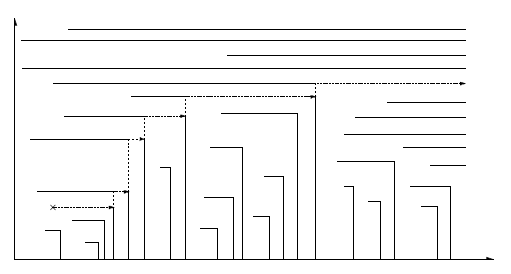
\includegraphics{insert.png}}
  \caption{The $Insert(t, ``insert(k)$'') operation causes a cascade of changes of delete times, and one insertion into $Q_0$. \cite{dil}}
  \label{fig:insert}
\end{figure*}

\begin{figure*}[h]
  \centering
  \leavevmode
  \scalebox{.5}{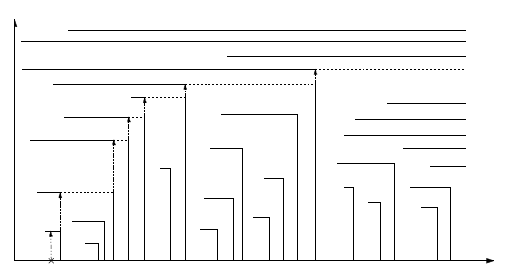
\includegraphics{delete.png}}
  \caption{The $Insert(t, ``delete$-$min()$'') operation causes a cascade of changes of delete times, and one deletion into $Q_0$. \cite{dil}}
  \label{fig:delete}
\end{figure*}

We can perform all of these operations in $O(\lg m)$ worst-case, where $m$ is the total number of updates, present or retroactive, performed on the priority queue. We first store a balanced BST insertions keyed on insertion time. We augment each node of this tree with the max key $k' \notin Q_0$ over every node's subtree. This lets us find the maximum key among all elements inserted after a time $t'$ but not in $Q_0$ in $O(\lg m)$ time. We can also find the minimum key among all elements inserted before a time $t'$ and still in $Q_0$ in the same runtime if we maintain in every node the minimum of all keys in its subtree still in $Q_0$. These are useful for operations 1 and 2, and 3 and 4, respectively.\\
\\
To find the last bridge before $t$ or the first bridge after $t$, we maintain a list of updates which we store in a modified $(a,b)$-tree developed by Fleischer \cite{fleischer}. If we assign a weight of 0 to $insert(k)$ for $k \in Q_0$, +1 to $insert(k)$ for $k \notin Q_0$, and -1 for $delete$-$min()$, every bridge in the tree corresponds to a prefix sum of 0. This allows us to find bridges in $O(\lg m)$ time, which we use for every operation.

\bibliography{mybib}
%\bibliographystyle{alpha}

\begin{thebibliography}{77}

\bibitem{fks}
M. Fredman, J. Koml\'{o}s, E. Szemer\'{e}di,
\emph{Storing a Sparse Table with $O(1)$ Worst Case Access Time},
Journal of the ACM, 31(3):538-544, 1984.

\bibitem{brodal}
Gerth St�lting Brodal: \emph{Partially Persistent Data Structures of Bounded Degree with Constant Update Time}. Nord. J. Comput. 3(3): 238-255 (1996)

\bibitem{dil}
Erik D. Demaine, John Iacono, Stefan Langerman: \emph{Retroactive data structures}. SODA 2004: 281-290

\bibitem{dietz}
Paul F. Dietz, Daniel Dominic Sleator: \emph{Two Algorithms for Maintaining Order in a List} STOC 1987: 365-372

\bibitem{dietz1}
Paul F. Dietz: \emph{Fully Persistent Arrays (Extended Array)}. WADS 1989: 67-74

\bibitem{dsst}
James R. Driscoll, Neil Sarnak, Daniel Dominic Sleator, Robert Endre Tarjan: \emph{Making Data Structures Persistent}. J. Comput. Syst. Sci. 38(1): 86-124 (1989)

\bibitem{kot}
Haim Kaplan, Chris Okasaki, Robert Endre Tarjan: \emph{Simple Confluently Persistent Catenable Lists}. SIAM J. Comput. 30(3): 965-977 (2000)

\bibitem{fiat}
Amos Fiat, Haim Kaplan: \emph{Making data structures confluently persistent}. J. Algorithms 48(1): 16-58 (2003)

\bibitem{okasaki}
Chris Okasaki: \emph{Purely Functional Data Structures}. New York: Cambridge University Press, 2003.

\bibitem{fhm}
Gudmund Skovbjerg Frandsen, Gudmund Skovbjerg Frandsen, Peter Bro Miltersen: \emph{Lower Bounds for Dynamic Algebraic Problems}. Information and Computation 171(2): 333-349 (2001)

\bibitem{fleischer}
Rudolf Fleischer: \emph{A Simple Balanced Search Tree with $O(1)$ Worst-Case Update Time}. Int. J. Found. Comput. Sci. 7(2): 137-150 (1996)

\end{thebibliography}

\end{document}
